% !TEX root = ../EDBT.tex
Traditional business intelligence is rapidly evolving to adopt modern big-data analytics architectures based on the concept of a `data lake', where, rather than  first integrating multiple historical data from diverse sources into a common star schema via extraction-transformation-load operations, the datasets are maintained in their raw form. This leads to a number of challenges; for example, dealing with incongruous join keys between different datasets. 

In this paper, we focus on a problem of fusion of information about consumer products, such as sales, market share, etc., which is spread across disparate databases belonging to different organizations, across which a product is \textit{not} identifiable via a common key. For example, a \textit{Global database (DB)}
might track overall market-share of global product categories. On the other hand, each \textit{Local DB} might track sales data within a geography 
using local-product-ids along with other characteristics, but \textit{not} the global category-id. As a result, an analytical task such as comparing the
sales of product categories within each geograpy against their global market share becomes difficult due to the lack of a natural join attribute between the databases.
(Note that the same product might be characterized using different attributes in different countries, including also textual \textit{description} of products entered manually by retailers, e.g., for carbonated drinks it usually contains information of brand, size, material used, packaging etc.) 

% \begin{figure}
% \centering
% \includegraphics[width=65mm]{Figures/local-char}
% \vspace{4pt}
% \caption{Local characteristics of the same product across four geographies and its corresponding global characteristics}
% \vspace{-18pt}
% \label{fig:local}
% \end{figure}

One way to perform analysis across disparate databases is by mapping records in each \textit{Local DB} to their corresponding global attributes (e.g., `category'
in the example above). However, preparing such mappings is a huge manual and complicated task because: a)~The cardinality (number of possible values) of local and global characteristics varies from tens to thousands, and b)~Uncertainty in the semantics of local characteristics of the same product from different geographies, leading to confusion in identifying the product category, even by human annotators.
 
Our aim is to help reduce cost of the operational process of creating and maintaining such global references by reducing manual workload via automation
via modern data-lake architecture that include automated fusion of federated databases. Our goal is to either make high confidence predictions, or abstain from making any prediction so that such records can be sent to human annotators. We want to minimize the number of such abstentions while maximizing the precision of the predictions.

\textbf{\textit{Attribute Fusion using Record Matching}}:
Consider two databases (see Figure~\ref{fig:Prob1}): a) \textit{Local DB($L$)} with each product $l$ having local characteristics $L_1, L_2,..., L_M$, e.g., flavor, brand, etc., and retailer descriptions ($D_i$), and b)~a \textit{Global DB($G$)} having $K$ global characteristics. The problem at hand is thus a \textit{record matching} problem where products in local database are to be mapped to global characteristic values (e.g. `category', or `global brand' etc.). 

Note that our objective is only to reconcile performance metrics (such as volume sales and market-share) across databases for each global characteristic \textit{independently}, e.g., sales vs market-share for each category, or alternatively each global brand, etc.
We can achieve this by solving $K$ different record matching problems,
as shown in Figure~\ref{fig:Prob1}: For each product, we shall predict each of the $K$ global characteristics
given local characteristics and retailer descriptions separately, as $\arg\max_j P(G_j | L_1, ..., L_M, D_i)$.

In this paper: a)~We address the problem of automating attribute fusion across diverse data sources that do not share a common join key.
b)~We augment traditional, fundamentally unsupervised text-similarly techniques with supervised, Bayesian network models in a confidence-based ensemble for automating the mapping process.
c)~Our approach additionally delivers confidence bounds on its predictions, so that human annotation can be employed when needed.
d)~We test our approach in a real-life market research scenario. We also compare it with available techniques \cite{christen2008febrl} and demonstrate that our approach outperforms FEBRL \cite{christen2008febrl}.
e) We illustrate how our approach has been integrated into a data-fusion platform\cite{singh2016visual} specifically designed to manage data-lakes containing disparate databases.

\textbf{Related Work:} Record linkage has been usually addressed via two categories of approaches, learning-based and non-learning based~\cite{kopcke2010evaluation}. Learning-based approaches such as FEBRL\cite{christen2008febrl} that uses SVM to learn a weighted combination
of similarity matching techniques followed by unsupervised matching, MARLIN~\cite{bilenko2003adaptive} uses similarity measures Edit Distance and Cosine and several learners. In non-learning based approaches, PPJoin+\cite{xiao2011efficient} is a single-attribute match approach using sophisticated filtering techniques for improved efficiency, and FellegiSunter\cite{fellegi1969theory} evaluates three of the similarity measures Winkler, Tokenset, Trigram. In\cite{poon2016ensemble}, an ensemble approach of two non-learning algorithms Fellegi-Sunter and Jaro-Wrinkler has been presented for record-linkage. In contrast, we use a confidence based ensemble approach that combines supervised learning using a Bayesian network model together with a non-learning based textual model.
Our approach also produces confidence bounds on the predictions that help to decide reliability of prediction.

\begin{figure}
\centering
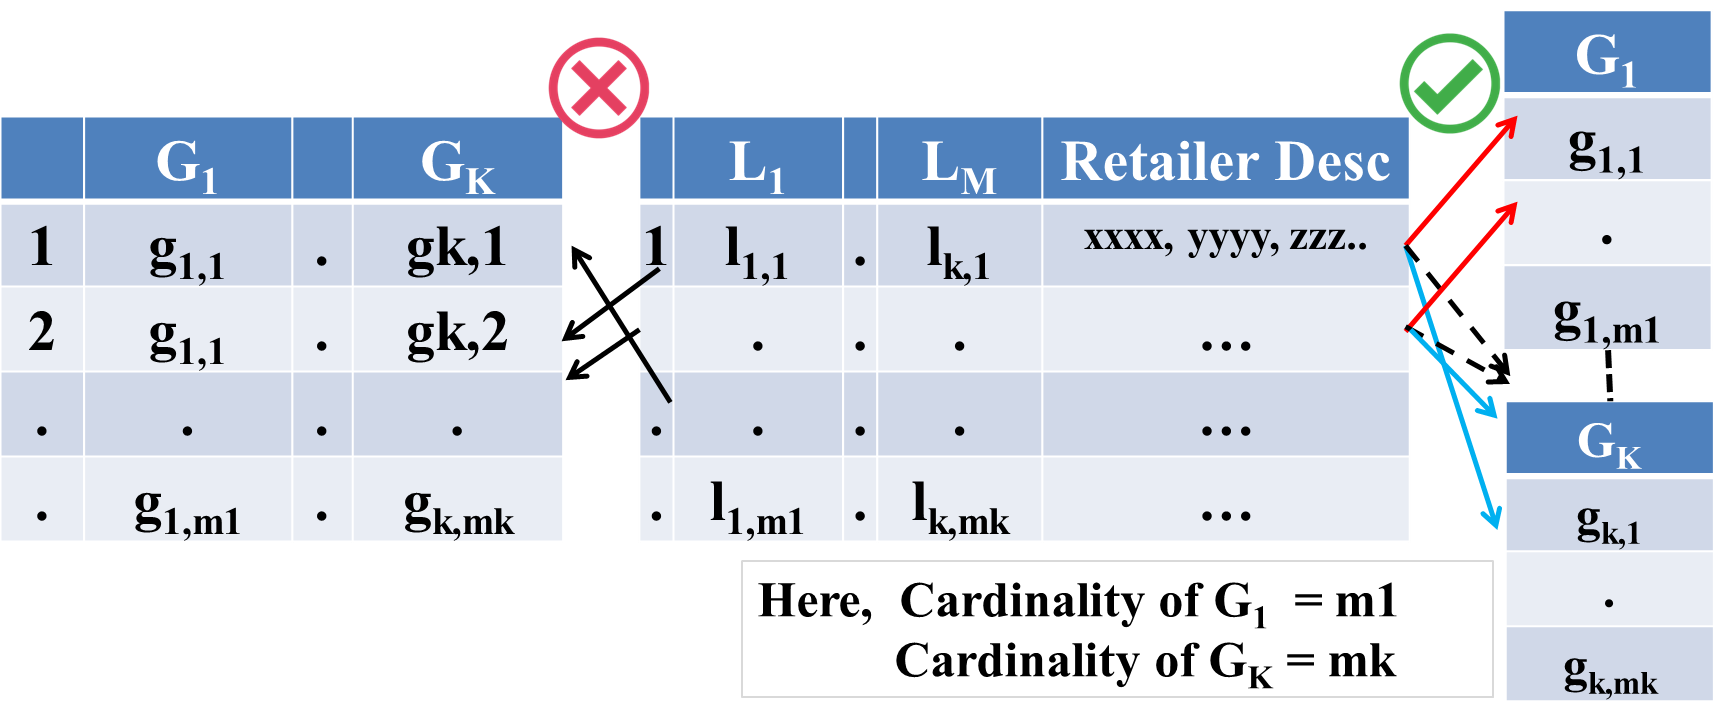
\includegraphics[width=120mm]{Figures/Prob-combine}
%\vspace{-2pt}
\caption{Local and Global Database}
%\vspace{-16pt}
\label{fig:Prob1}
\end{figure}

% \begin{figure}
% \centering
% \includegraphics[width=65mm]{Figures/Prob-2}
% %\vspace{-8pt}
% \caption{$K$ record matching problems}
% %\vspace{-12pt}
% \label{fig:Prob2}
% \end{figure}




% \subsection{Paper Organization}
% The remainder of the paper is organized as follows: We begin with overview of our approach in Section~\ref{sec:over} followed by the detail description of BGM model in Section~\ref{sec:BGM}, where we present Bayesian approach to predict global characteristics, which includes tree-based structure learning, Bayesian parameter learning, and Bayesian inference using SQL databases. The TIR model to predict global characteristics using textual descriptions is presented in Section~\ref{sec:tir}. Next, we present an ensemble approach of these two models in Section~\ref{sec:ensemble}, where we calculate confidence of the prediction from each model and use it to combine predictions from both models. Results of our techniques and integrated approach using real world 
% data are presented in Section~\ref{sec:experiment}. Finally, after the brief description of related work in Section~\ref{sec:related}, we conclude in Section~\ref{sec:conc} highlighting the prevalence of the problem we have addressed.